% !TeX spellcheck = da_DK
\section{Følger af apopleksi }
Apopleksi kan forekomme pludseligt og dermed uden, at den ramte kan forberede sig på følgerne. Dette er modsat andre sygdomme, såsom diabetes, sclerose og KOL, hvor progressionen ofte sker gradvist. Der kan opstå psykiske konsekvenser forårsaget af hæmoragisk eller iskæmisk apopleksi som f.eks. depression eller angst, hvilket bl.a. går udover patientens lyst til at komme tilbage til sin normale hverdag. Følgerne kan derfor have indflydelse på patientens fysiske og mentale tilstand. \cite{Muus2008} Udover de psykiske konsekvenser giver apopleksi andre følger, som afhænger af, hvilken del af encephalon der rammes, og hvor omfangsrig hjerneskaden er. Omfanget afhænger af tiden, hvor en del af encephalon ikke får ilt, størrelse af den eventuelle blødningen og trykket i arterien \cite{Michael-Titus2010}. 
% ALT DETTE STÅR I INDLEDNINGEN - 75.000 mennesker over 18 år levede i 2011 med følger efter et slagstilfælde \cite{Hjernesagen2015}. Dette tal forventes at være stigende i takt med, at der kommer flere ældre \cite{Sagen2014}. Antallet der dør af hjerneskader har været stagneret de sidste 10 år før 2011, hvor 14 \% døde inden for 30 dage[3]. Det vil derfor kunne forventes, at der er flere, som kommer ud for en hjerneskade og vil have mén herefter, hvilket gør det vigtigt at fokusere på rehabiliteringen for at kunne genoptræne de forskellige kropslige og mentale mangler.

\subsection{Sensoriske og motoriske skader} %Sproglige, sensoriske og motoriske skader
%De sproglige konsekvenser fra apopleksi kaldes afasi. Afasi opleves efter en måned hos 20\% af de apopleksiramte og forekommer oftest ved skade i venstre temporal- og frontallap. De sproglige følger af apopleksi kan skade funktionen til at skrive og tale, men også evnen til at forstå og læse andres tale og skrift. I hvilken grad de sproglige funktioner er berørt kan variere mellem de enkelte patienter, da nogle oplever enkelte formuleringsproblemer, mens andre oplever global afasi. Global afasi gør, at de ramte i nogle tilfælde er helt ude af stand til at kommunikere verbalt eller kun kan fremsige enkelte ord med en vis usikkerhed omkring ordenes betydning.
%De sproglige konsekvenser kan midlertidig bedres med tiden, og flere patienter opnår et kommunikationsniveau, som gør det muligt at begå sig i hverdagen.\cite{Muus2008} \\
De sensoriske og motoriske konsekvenser er de hyppigst forekommende følger hos apopleksiramte og kan medføre problemer med udførsel af orienterende handlinger. \cite{Kruuse2015a,DSfA2009}  De sensoriske og motoriske funktioner har indflydelse på hinanden, da der ofte anvendes sanser og motorik til udførsel af forskellige funktioner \cite{Nichols1997}.  \\
Som tidligere nævnt i afsnit \ref{HjerneSenMot} kan apopleksi skade sensoriske såvel som motoriske funktioner, som kan ses på \figref{Enc} på side \pageref{Enc} .\\

\noindent Symptomerne på sensoriske følger kan bl.a. være:
\begin{itemize}
  \item Agnosi: Manglende evne til at genkende genstande på trods af klare sanseindtryk af genstanden. Der er flere former for agnosi, som har indflydelse på det at kunne genkende ansigter, lyde og legemesdele \cite{Redaktionen2015}. 
 \item Agnosognosi: Manglende sygdomserkendelse, hvilket f.eks. kan opleves ved, at patienten nægter sin halvsidige lammelse. I nogle tilfælde kan patienten oplyse om sin lammelse men vil stadig ikke erkende, at den er der \cite{Pedersen1999}.
\end{itemize}
Apopleksipatienterne kan derfor både have problemer med forholdet mellem egen krop og objekter omkring sig, afstandsbedømmelse samt kropsdelenes indbyrdes forhold \cite{Kruuse2015a,DSfA2009}. Derudover kan de sensoriske følger have indflydelse på motoriske følger, som f.eks. hvis encephalon ikke kan genkende og omdanne signalerne fra sansereceptorer til motoriske bevægelser. \cite{Martini2012,Nichols1997}. \\

\noindent Symptomerne på motoriske følger kan bl.a. være:
\begin{itemize}
  \item Parese: Nedsat kraft i muskulaturen, hvilket vil sige, at der er bevægelse men i mindre grad end normalen. Hvis der er nedsættelse i halvdelen af kroppen kaldes det hemiparese \cite{Kruuse2015a}.
  \item Paralyse: Ingen bevægelse i hele muskulaturen, hvilket vil sige, at kroppen er fuldstændig lammet. \cite{Vistrup2015}
  \item Ataksi: Manglende evne til koordinering af muskelbevægelser. Dette sker ofte pga. sygdom i cerebellum \cite{Redaktionen2015a}. 
\end{itemize}
Som følge af et apopleksitilfælde kan motoriske mén medføre begrænsninger i bevægelse ift. præcision, generel stivhed, opstart af gang, hurtige og spontane bevægelser samt rystelser. Alle disse følger har betydning for patientens balance og kan give udfordringer for patienten ift. at kunne sidde, stå eller gå. \cite{Kruuse2015a,DSfA2009}

\subsubsection{Balance}\label{BalanceAfsnit}
En sensorisk og motorisk skade kan lede til balanceproblemer, da både kroppens sanser samt motorik hjælper til opretholdelse af balance. Balancen er vigtig for mennesket, eftersom den opretholder kropsstillingen vha. ubevidste bevægelser og gør bevægelse muligt uden fald. For at opretholde balancen bliver kropsvægten så vidt mulig fordelt omkring kroppens akse og de vægtbærende legemer, herunder fødder i oprejst position og gluteal musklerne i siddende position. \cite{Nichols1997} \\
Balancen er et komplekst system, da proprioceptorer og sansereceptorer samarbejder om at sende balanceinformation til encephalon, hvor den bearbejdes. Samarbejdet mellem receptorerne er illustreret på \figref{flowbalance1}. Proprioceptorerne kontrollerer muskler, sener og leddenes position, dvs. de styrer ubevidste bevægelser. \cite{Martini2012} Sansereceptorer fra vestibulen og øjne opfanger sanseindtryk. Proprioceptorer og sansereceptorer udgør de sensoriske indput, som videresendes til områder i cerebral cortex, cerebellum og til centre i hele truncus encephalicus. Disse områder bearbejder balanceinformationen for at konkludere den fysiske position af kroppen og dens lemmer. Herved opretholdes balancen. \cite{Karnath2003,Martini2012} Proprioceptorer og sansereceptorerne, samt hvor de findes, uddybes i bilag \ref{app-Balance}.

\begin{figure}[H]
	\centering
	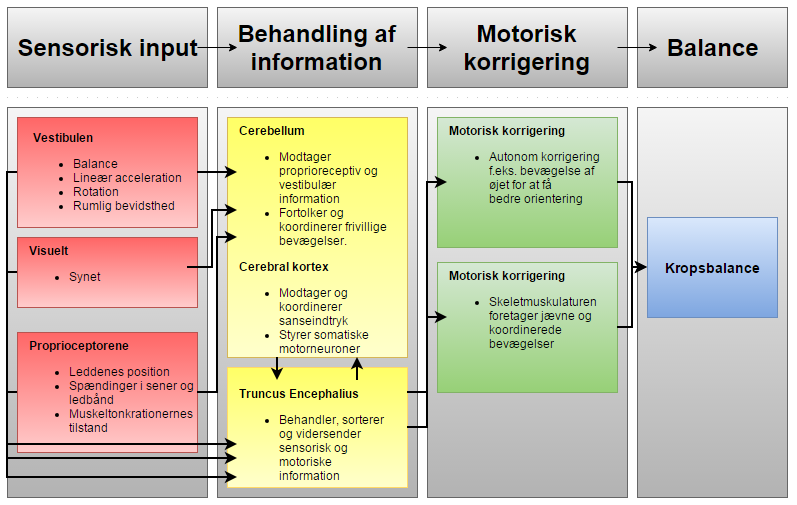
\includegraphics[scale=0.55]{figures/bProblemanalyse/Balance-Flowdiagram.png}
	\caption{På flowdiagramet ses, hvordan sansereceptorer og propioreceptorer samarbejder for at opretholde kropsbalancen \cite{watson2015}.}
	\label{flowbalance1}
\end{figure}

Apopleksipatienter oplever balanceproblemer, da samarbejdet mellem proprioceptorerne og sansereceptorer er svækket, og de behandlende centre i encephalon er skadet. \cite{Martini2012} En rask persons krop svajer som udgangspunkt omkring seks til syv grader i lateral retning \cite{Wang2010,Huo1999}. Grænsen for hvornår balancen ikke kan opretholdes er individuel og påvirkes af forskellige faktorer såsom alder og styrke \cite{Huo1999}. Det kan derfor være vanskeligt at definere en værdi for denne grænse. \\ 
Balancen har betydning for den siddende, stående og gående position, og de forskellige positioner afhænger af hinanden, hvilket kan give begrænsninger i hverdagen. Problemer ved opretholdelse af nævnte positioner giver øget risiko for faldulykker. \cite{Karnath2003} 

Et eksempel på, hvordan balancen påvirkes, er Pusher Syndrom. Dette er en lidelse, hvor halvsidigt lammede patienter aktivt skubber deres kropsvægt mod den lammede kropsside, hvilket er illustreret på \figref{pusher}. Lidelsen kan opstå som følge af både højre- og venstresidig hjerneskade. Patienter med Pusher Syndrom registrerer ikke, at deres krop hænger, hvilket kan være med til at besværliggøre funktioner i dagligdagen og giver øget risiko for faldulykker i både stående, gående og siddende stilling. \cite{Karnath2003} 

\begin{figure}[H]
	\centering
	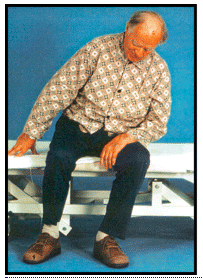
\includegraphics[scale=0.9]{figures/bProblemanalyse/Pusher.png}
	\caption{På billedet ses en patient med pusher syndrom. Det ses tydeligt, at patienten hænger til sin venstre side med kroppen \cite{Karnath2003}.}
	\label{pusher}
\end{figure}

\subsubsection{Neglekt}
Neglekt er en sensorisk og motorisk skade, og derfor kan sygdommen forekomme visuelt, kropsligt eller kombineret. \fxnote{NTK: http://gade.psy.ku.dk/bogkap/neglekt.htm er god at læse før eksamen} Der er mange former for neglekt, hvor graden kan variere, som kan forekomme samtidigt \cite{Sundhed.dk2014}. Det anslås, at $25\%$ af apopleksipatienterne i 2009 var ramt af neglekt. \cite{Sundhedsstyrelsen2009}

Ved visuel neglekt kan patienten bl.a. mangle sanseindtryk fra den påvirkede side af kroppen. Patienten er eksempelvis ikke opmærksom på den ene side af teksten, når vedkommende skal læse, selvom synet er normalt. Derudover kan patienten opleve kun at spise fra den ene del af tallerkenen, eftersom encephalon ikke registrerer den anden halvdel. \cite{Sundhed.dk2014}\\
Ved den kropslige neglekt kan patienten have manglende kropsbevidsthed. Patienten har ofte normal følelse i den syge side af kroppen - indtrykkene bemærkes, men registres ikke i encephalon. Det kan komme til udtryk i, at patienten glemmer at klæde den syge side af kroppen ordentligt på eller kun barbere halvdelen af ansigtet. En alvorlig følge af kropslig neglekt kan være, at patienten udfører ubevidst skade på sig selv. Patienten kan f.eks. støde ind i ting med den syge side eller ikke være opmærksom på, at benene ikke kan bære kropsvægten og derved miste balancen. Af denne grund kan der på længere sigt forekomme ergonomiske skader andre steder i kroppen. \cite{Kruuse2015a}

\subsection{Personlige følger} \label{Personlige_foelger}
Dette afsnit er baseret på hjerneskader generelt. Dvs. det ikke er sikkert, at apopleksi er årsagen, men det antages, at de samme udfordringer gør sig gældende hos personer, der får hjerneskader af apopleksi. Derudover skal det noteres, at det ikke er sikkert, at en patient får følger af apopleksi.

Personer, der rammes af en hjerneskade, beskriver hjerneskaden som et brud i deres liv, som de skal lære at forholde sig til. Det kan tage tid for patienterne at indse, at de er ramt af en sygdom. Patienten er ikke i stand til at udføre de samme opgaver som tidligere f.eks. grundet balancebesvær, hvilket har betydning den ramtes identitet, aktivitet og sociale relationer. Kroppens funktionsændringer gør, at den ramte kommer til at leve et mere inaktivt og hjemmeorienteret liv end før. En yngre patient er mere ramt af denne forandring ift. en ældre patient. Dette kan bl.a. skyldes vanskeligheden i at opretholde sociale relationer og begå sig i hverdagen. Apopleksiramte kan derudover opleve en kropsspaltning, hvor kroppen opleves som et fremmedobjekt. \cite{Sundhedsstyrelsen2010,Badke2009}

Der findes ikke synlige vanskeligheder for patienter med hjerneskade som f.eks. besvær med hukommelse, læsning og regning. Disse vanskeligheder har også en indflydelse på patientens selvopfattelse og  kan derved være med til at nedsætte livskvaliteten for den enkelte. \cite{Sundhedsstyrelsen2010} 


%\subsection{Identitet}
%En hjerneskadets identitet ændres, da patienten ikke er i stand til at udføre de samme opgaver som tidligere. Derfor bliver den hjerneskadede nødt til at skabe en ny identitet, hvilket for mange kan være svært. Kroppens funktionsændringer gør, at den ramte kommer til at leve et mere inaktivt og hjemmeorienteret liv end før. En yngre patient er mere ramt af denne forandring i forhold til en ældre patient. Apopleksiramte kan derudover opleve en kropsspaltning, hvor kroppen opleves som et fremmet objekt. Et objekt, som kan være svært at styre og ikke gør, som patienten vil.\cite{Sundhedsstyrelsen2010} 

%Der findes skjulte vanskeligheder for patienter med hjerneskade. Disse omfatter vanskelighed med hukommelse, læsning, regning samt andre færdigheder, der ikke er let synlige. Disse skjulte vanskeligheder har også en indflydelse på, hvordan patienten opfatter sig selv og kan være med til at nedsætte livskvaliteten for den enkelte.\cite{Sundhedsstyrelsen2010} 

%\subsection{Patienternes påvirkning}
%Alle de fysiske og mentale ændringer medfører, at det er svært for en hjerneskadet patient at vende tilbage til sit gamle hverdagsliv. Forandringerne gør det svært at udføre almindelige huslige pligter, såsom rengøring og personlig pleje. De ramte oplever det også som en svær oplevelse at vende tilbage på arbejde. Dette skyldes, udover de kropslige og mentale ændringer, også den træthed, der kan opleves. Det er derfor vigtigt at føle sig værdsat på jobbet. Den hjerneskadede patient skal vende tilbage til sine sociale relationer. Dette kan opleves som en meget hård opgave pga. de forandringer, kroppen har gennemgået. Det ses imidlertid, at familierelationerne bliver tættere, mens relationerne til vennerne bliver mindre. Dette er et problem, da gode relationer kan være med til at forbedre rehabiliteringsprocessen og dermed gøre, at den hjerneskadede patient hurtigere kan komme tilbage til et normalt liv.\cite{Sundhedsstyrelsen2010}

%Ud fra  det ovenstående kan det konkluderes, at hjerneskadede patienter, heriblandt apopleksiramte, oplever nedsat livskvalitet pga. deres sygdom. Dette kan også ses ved, at apopleksipatienter har dobbelt så stor selvmordsrate som baggrundsbefolkningen. Derudover nævner 16\% af apopleksi patienter, at deres livskvalitet er dårlig, 46\% syntes den er nogenlunde, mens 38\% synes den er god. Den nedsatte livskvalitet er noget der kan føre til vanskeligheder senere i livet, hvilket selvfølgelig skal forsøges undgået. En forbedret livskvalitet kan skabes ved hurtigere rehabilitering eller forbedret kropslig funktion, som den apopleksiramte patient mistede ved hjerneskaden.\cite{Sundhedsstyrelsen2010}